Além da verificação da eficiência dos controladores atuando sobre o sistema para o qual foram projetados, eles foram testados num sistema em que um dos parâmetros foi acrescido de mais de 100 \%, com a massa passando de 2,3 kg para 5 kg.

A resposta dos controladores fuzzy e neuro-fuzzy para altitude do drone nessas circunstâncias são mostradas nas Figuras \ref{fig:altitude_z_zdot_5kg} e \ref{fig:altitude_z_zdot_5kg_closer}, sendo que esta segunda é apenas uma forma melhor de comparar a ação dos dois controladores. Como se pode perceber, ambos os controladores levaram à estabilização do sistema, sendo que desta vez cada um obteve desempenho melhor sob determinados aspectos. No controle da posição vertical $z$, o neuro-fuzzy apresentou tempo de convergência 57\% maior, em parte causado por uma sobrelevação, que não foi apresentada pelo fuzzy. Em contrapartida, o neuro-fuzzy apresentou uma menor variação, a reduzindo em 20\% se comparado ao fuzzy. Com relação à velocidade $\dot{z}$, o controlador neuro-fuzzy apresentou aumento de 23\% no tempo de convergência, mas melhorou o sistema nos quesitos variação e sobrelevação, as reduzindo em 16\% e 33\%, respectivamente. Esses resultados apontam que o quadrotor, quando submetido ao controle neuro-fuzzy, apresentou movimentos mais suaves até ter sua altitude estabilizada, apesar de ter sido necessário mais tempo para que ela ocorresse.

%sendo que o fuzzy desta vez obteve melhor desempenho sobre $z$, sendo isento de oscilações, diferentemente do neuro-fuzzy, o que representa que, no caso do controle neuro-fuzzy, o drone passou do ponto da posição inicial e depois teve que retornar a ele. Já com relação a $\dot{z}$, o neuro-fuzzy apresentou menor sobrelevação, apesar de oscilar levemente,o que indica que o quadrotor apresentou movimentos mais suaves até ter sua altitude estabilizada.

% Altitude m=5
\begin{figure}[!htb]
    \centering
    \caption{Comparação da resposta das saídas $z$ e $\dot{z}$ no controle de altitude fuzzy e neuro-fuzzy para o sistema com massa $m=5kg$}
    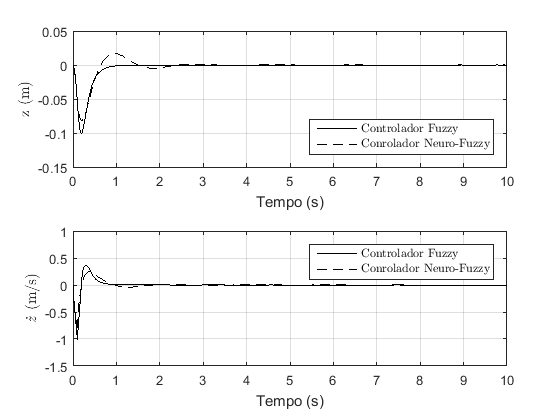
\includegraphics[width=0.8\textwidth]{./04-figuras/resultados/novos/altitude_z_zdot_5kg}
    \label{fig:altitude_z_zdot_5kg}
\end{figure}

% Altitude m=5, closer
\begin{figure}[!htb]
    \centering
    \caption{Comparação em mais detalhes da resposta das saídas $z$ e $\dot{z}$ no controle de altitude fuzzy e neuro-fuzzy para o sistema com massa $m=5kg$}
    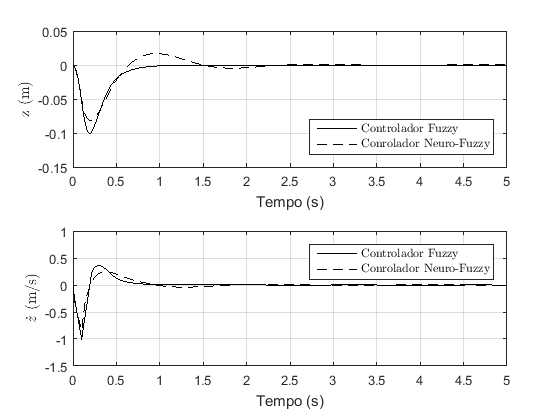
\includegraphics[width=0.8\textwidth]{./04-figuras/resultados/novos/altitude_z_zdot_5kg_closer}
    \label{fig:altitude_z_zdot_5kg_closer}
\end{figure}


% -------------------  ATITUDE ---------------

Por fim, as Figuras \ref{fig:atitude_phi_phidot_5kg_40s} e \ref{fig:atitude_theta_thetadot_5kg_40s} mostram os resultados obtidos pelos controladores de atitude no sistema com massa $m=5$ $kg$. Percebe-se que mais uma vez o sistema convergiu ao seu estado de estabilidade com os ângulos nulos e velocidades angulares também nulas, representando que o quadrotor, após a ação de controle, tanto fuzzy quanto neuro-fuzzy, fica estável e com orientação plana\footnote{i.e\ paralela ao plano XY}.

As Figuras \ref{fig:atitude_phi_phidot_5kg_10s} e \ref{fig:atitude_theta_thetadot_5kg_10s} mostram em mais detalhes as repostas obtidas pelos controladores sobre a atitude do sistema com massa $m=5$ $kg$. A partir delas, nota-se que mais uma vez o controlador neuro-fuzzy apresentou desempenho levemente superior ao fuzzy. Sobre os ângulos $\phi$ e $\theta$, a convergência ocorreu 3\% mais rapidamente e a variação apresentada reduziu 14\%. Já sobre as velocidades angulares $\dot{\phi}$ e $\dot{\theta}$, a redução de tempo de convergência com o neuro-fuzzy foi de 2\%, mantendo a mesma sobrelevação e variação oferecidas pelo fuzzy. Com isto, mais uma vez o controle neuro-fuzzy fez com que o ângulo máximo de inclinação do quadrotor fosse inferior ao alcançado pelo sistema controlado pelo fuzzy,e além de reduzir o tempo necessário para sua estabilização definitiva.

%com menor variação do sistema e convergência em tempo ligeiramente menor.
%
%A partir das Figuras \ref{fig:atitude_phi_phidot_2kg_10s} e \ref{fig:atitude_theta_thetadot_2kg_10s}, que mostram as respostas obtidas em mais detalhes, pode-se ver que, mais uma vez o controlador neuro-fuzzy mais uma vez teve desempenho superior ao fuzzy, fazendo com que os ângulos $\phi$ e $\theta$ convergissem 2\% mais rápido, além de reduzir suas variações em 13\%. Com relação às velocidades angulares $\dot{\phi}$ e $\dot{\theta}$, o neuro-fuzzy foi capaz de reduzir o tempo de convergência em 3\%, não afetando a variação nem a sobrelevação apresentada pelo sistema quando estabilizado pelo controlador fuzzy. Desta forma, verifica-se que o controle neuro-fuzzy levou o sistema a uma menor variação, representando que o ângulo máximo de inclinação alcançado pelo drone é menor e corrigido mais rapidamente.
% Atitude m=5
%phi
\begin{figure}[!htb]
    \centering
    \caption{Comparação da resposta das saídas $\phi$ e $\dot{\phi}$ no controle de atitude fuzzy e neuro-fuzzy para o sistema com massa $m=5kg$}
    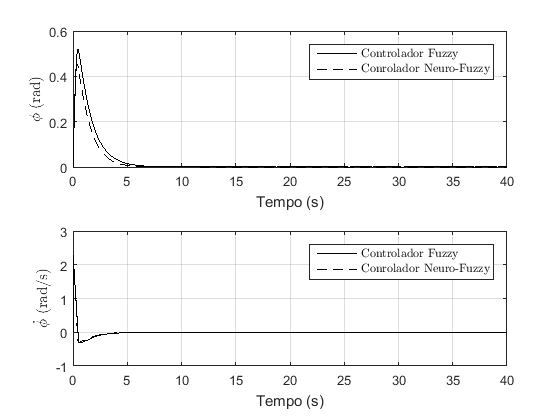
\includegraphics[width=0.8\textwidth]{./04-figuras/resultados/novos/atitude_phi_phidot_5kg_40s}
    \label{fig:atitude_phi_phidot_5kg_40s}
\end{figure}

%theta
\begin{figure}[!htb]
    \centering
    \caption{Comparação da resposta das saídas $\theta$ e $\dot{\theta}$ no controle de atitude fuzzy e neuro-fuzzy para o sistema com massa $m=5kg$}
    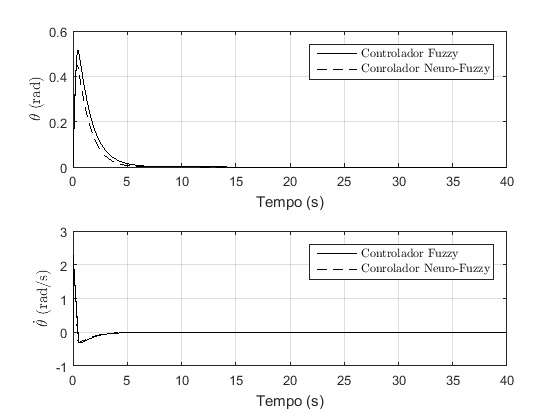
\includegraphics[width=0.8\textwidth]{./04-figuras/resultados/novos/atitude_theta_thetadot_5kg_40s}
    \label{fig:atitude_theta_thetadot_5kg_40s}
\end{figure}



\begin{figure}[!htb]
    \centering
    \caption{Comparação da resposta das saídas $\phi$ e $\dot{\phi}$ no controle de atitude fuzzy e neuro-fuzzy para o sistema com massa $m=5kg$}
    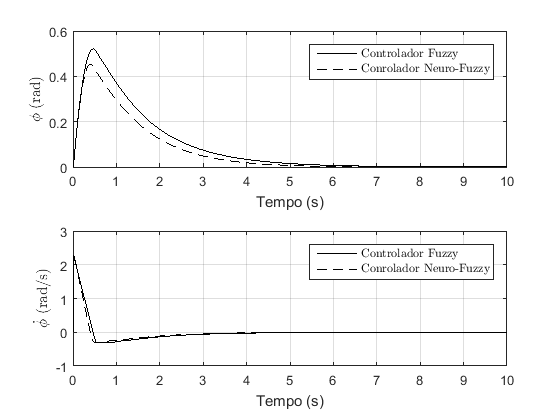
\includegraphics[width=0.8\textwidth]{./04-figuras/resultados/novos/atitude_phi_phidot_5kg_10s}
    \label{fig:atitude_phi_phidot_5kg_10s}
\end{figure}

%theta
\begin{figure}[!htb]
    \centering
    \caption{Comparação da resposta das saídas $\theta$ e $\dot{\theta}$ no controle de atitude fuzzy e neuro-fuzzy para o sistema com massa $m=5kg$}
    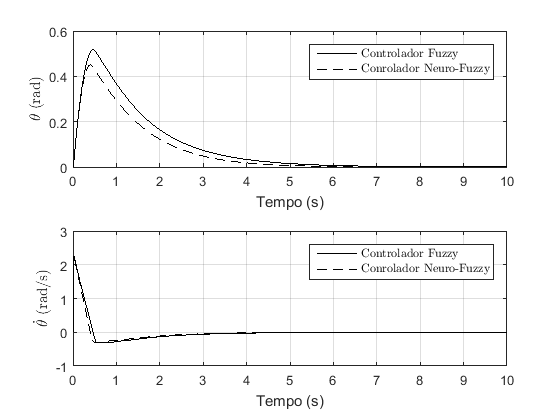
\includegraphics[width=0.8\textwidth]{./04-figuras/resultados/novos/atitude_theta_thetadot_5kg_10s}
    \label{fig:atitude_theta_thetadot_5kg_10s}
\end{figure}




